\documentclass[a4paper,man,natbib,donotrepeattitle, apacite]{apa6}
\usepackage{authblk}% for multiple authors
\usepackage{tabularx} % to create tables in methods

\usepackage[english]{babel}
\usepackage[utf8x]{inputenc}
\usepackage{amsmath}
\usepackage{graphicx}
\usepackage[colorinlistoftodos]{todonotes}
\geometry{reset, letterpaper, height=9in, width=7in, hmarginratio=1:1, vmarginratio=1:1, marginparsep=0pt, marginparwidth=0pt, headheight=15pt}
\usepackage{tikz}
\usepackage{wrapfig}
\usepackage{amssymb}
\usepackage{amsmath,subcaption,caption}
\usepackage{ifxetex,ifluatex}
\usepackage{fixltx2e,authblk} % provides \textsubscript
\usepackage{lmodern}
\usepackage[T1]{tipa}
\usepackage{longtable,booktabs}


\title{\LARGE Practice and experience predict coarticulation in child speech}

\shorttitle{Coarticulation in child speech}

\usetikzlibrary{shapes.geometric, arrows,backgrounds,fit,positioning}

\author[1,2]{\large Margaret Cychosz}
\author[3]{Benjamin Munson}
\author[1]{Jan R. Edwards}

\affil[1]{\small Department of Hearing and Speech Sciences, University of Maryland, College Park}
\affil[2]{Center for Comparative and Evolutionary Biology of Hearing, University of Maryland, College Park}
\affil[3]{Department of Speech-Language-Hearing Sciences, University of Minnesota, Twin Cities}

\affiliation{} % to remove weird affiliation

\clearpage
\authornote{Author to whom correspondence should be addressed: Margaret Cychosz, 0100 Samuel J. LeFrak Hall, University of Maryland, College Park, College Park, USA, 20742. Email: mcychosz@umd.edu.}






\abstract{Much research in child speech development suggests that young children coarticulate more than adults. There are multiple, not mutually-exclusive, explanations for this pattern. First, children may coarticulate more because they are limited by immature motor control. Children might also coarticulate more because they initially represent phonological segments in larger, more holistic units such as syllables or feet. We tested these explanations by evaluating how  four-year-old children’s language experience and practice predict their coarticulation between adjacent segments in real words and paired nonwords. Children with larger vocabularies coarticulated less, especially in real words, though there were no reliable coarticulatory differences between real words and nonwords after controlling for word duration. Children who vocalized more throughout a daylong audio recording also coarticulated less. Quantity of child vocalizations was more predictive of the degree of children's coarticulation than a measure of receptive language experience, adult word count. Overall, these results suggest strong roles for children's phonological representations, as well as their immature motor control, for coarticulatory development.}

\keywords{speech development, speech production, coarticulation, phonology, word repetition, naturalistic recording}


\begin{document}
\setlength\parindent{24pt} % indent each paragraph



\maketitle

\setcounter{secnumdepth}{2} % number sections

\section{Introduction}

A long standing question in language development is whether the representation of linguistic forms differs between adults and children. Numerous experimental paradigms and techniques examining speech perception and lexical access (e.g. head-turn preference, eye-tracking), have addressed this question \cite{majoranoRelationshipInfantsProduction2014, storkelLexiconPhonologyInteractions2002,swingleyLexicalNeighborhoodsWordForm2002}. However, children’s own speech production has also been studied to shed light on the nature of their phonological representations \cite{fergusonWordsSoundsEarly1975,goffmanBreadthCoarticulatoryUnits2008,nittrouerEmergencePhoneticSegments1989,nittrouerHowChildrenLearn1996,noiraySpokenLanguageDevelopment2019,noirayHowChildrenOrganize2018,redfordGrammaticalWordProduction2018,songEffectsCoarticulationMorphological2013,songDurationalCuesFricative2013,zharkovaCoarticulationIndicatorSpeech2011}. These works have demonstrated that speech production patterns, such as the duration, variability, and especially fluency of speech, can lend insight into speakers’ phonological representations and planning. 

One production metric that is frequently used to measure speech fluency in development is coarticulation, or the temporal and gestural overlap that results from producing two speech sounds in a sequence \cite{gerosaAnalyzingChildrenSpeech2006,goffmanBreadthCoarticulatoryUnits2008,zharkovaCoarticulationIndicatorSpeech2011}. Coarticulation is not simply noise in the speech signal. It conveys important auditory-acoustic information for speakers and listeners alike. Appropriate coarticulatory overlap, such as the ability to anticipate forthcoming speech segments, indicates mature, adult-like speech \cite{barbierWhatAnticipatoryCoarticulation2020,bradlowConfluentTalkerListeneroriented2002,whalenCoarticulationLargelyPlanned1990}. Children speak more slowly overall, and with less coordinated movement \cite{greenPhysiologicDevelopmentSpeech2000,goffmanRelationsSegmentalMotor2007,leeAcousticsChildrenSpeech1999}. It might then be logical to conclude that children coarticulate less than adults. Some studies have indeed concluded that children show less long-distance anticipatory coarticulation than adults, for example across syllable boundaries \cite{barbierWhatAnticipatoryCoarticulation2020}. However, a consensus is now growing that children actually coarticulate more than adults, both over longer distances (\citeNP{rubertusDevelopmentGesturalOrganization2018,rubertusVocalicActivationWidth2020}; cf. \citeNP{goffmanBreadthCoarticulatoryUnits2008}) and between adjacent segments within syllables \cite{nittrouerEmergencePhoneticSegments1989,nittrouerHowChildrenLearn1996,noirayBackFutureNonlinear2019,rubertusVocalicActivationWidth2020,zharkovaCoarticulationIndicatorSpeech2011,zharkovaSpatialTemporalLingual2014}. 

\subsection{The development of coarticulation}

A number of explanations have been offered for why children coarticulate between adjacent segments more than adults. Children’s coarticulation could reflect 1) low-level pressures upon speech due to the protracted development of fine motor control, 2) the phonological reorganization of speech from more holistic units, such as syllables, into phonemes, 3) domain-general cognitive pressures from children's limited working memory and planning capacities, or a combination of these explanations. 

First, children could coarticulate more because their fine motor control develops gradually throughout childhood and well into early adolescence \cite{barbierWhatAnticipatoryCoarticulation2020,kentAnatomicalNeuromuscularMaturation1976,perkellFiveDecadesResearch2013,walshArticulatoryMovementsAdolescents2002}. The spatiotemporal coordination of the lips and jaw, for example, undergoes significant development between ages two and six---younger children tend to rely more on vertical jaw movement, only learning to simultaneously coordinate both the lips and jaw with age \cite{greenPhysiologicDevelopmentSpeech2000}. Unsurprisingly, this motor control development has implications for children’s phonetic production, including coarticulation. For example, \citeauthor{zharkovaDynamicsVoicelessSibilant2018} (2018) measured coarticulation within /\textschwa sV/ and /\textschwa \textesh V/ sequences in children aged 7;0-13;0 and adults and found both that the ability to differentiate between /s/ and /\textesh/ increased with age and that the youngest children were most variable. The authors attribute these findings to the children’s developing control of the tongue, especially its coordination with the lips and jaw. \citeauthor{rubertusDevelopmentGesturalOrganization2018}(2018) likewise attribute 3;6-7;0 children’s coarticulation patterns---all children engaged in more V-V anticipatory coarticulation than adults---to protracted lingual coordination.           

Another reason younger children coarticulate more than adults and older children is if they initially represent language more holistically than adults, in units such as syllables, feet, or morae, instead of phoneme-sized segments. The exact unit of representation may vary by lexical item and depend upon the child's developmental stage \cite{davisEmergenceDiscretePerceptualMotor2019} as well as their familiarity with the phoneme sequence(s) or word in question. More familiar, frequent words likely have more segmental representations \cite{edwardsInteractionVocabularySize2004}, but representations may also be redundant: a given word may be encoded both holistically as well as segmentally, as is often argued to be the case even in adult phonology \cite{pierrehumbertPhoneticDiversityStatistical2003}. Overall, however, these larger speech units would be activated during children’s speech planning resulting in significant anticipatory effects of adjacent segments on one another.\footnote{The literature does, however, remain somewhat mixed on the directionality of coarticulatory development. Some studies have been unable to find a difference between adult and child coarticulation between adjacent segments \cite{katzAnticipatoryCoarticulationSpeech1991,noirayDevelopmentMotorSynergies2013,serenoDevelopmentalAspectsLingual1987,zharkovaDynamicsVoicelessSibilant2018}, while others have found that children coarticulate less \cite{kentSegmentalOrganizationSpeech1983}.} Anticipatory coarticulation between adjacent phones then decreases with age as phonological units reorganize into smaller segments in a phenomenon of child phonology often termed \textsc{Phonological Reorganization}  \cite{goodellAcousticEvidenceDevelopment1992,metsalaYoungChildrenPhonological1999,metsalaYoungChildrenPhonological1999,nittrouerEmergencePhoneticSegments1989,nittrouerHowChildrenLearn1996,noiraySpokenLanguageDevelopment2019,noirayHowChildrenOrganize2018,redfordGrammaticalWordProduction2018,zharkovaCoarticulationIndicatorSpeech2011}.\footnote{It is important to underscore how this phonological reorganization could play out differently cross-linguistically. Results from tests of phonological awareness in Mandarin-speaking children, for example, suggest that syllable and tone awareness are more important for character recognition than sub-syllabic awareness \cite{mcbride-changLevelsPhonologicalAwareness2004,shuPhonologicalAwarenessYoung2008a}. The developmental trajectories of phonological reorganization may then differ based on the language of exposure.} This phonological reorganization, children's advancement from more holistic to segmental speech representations, is driven by myriad factors including vocabulary growth \cite{metsalaSpokenVocabularyGrowth1998}, construction of (denser) phonological neighborhoods \cite{storkelInfluencePartwordPhonotactic2011}, and, starting around age 5, phonological awareness/literacy development \cite{metsalaYoungChildrenPhonological1999}. For example, vocabulary growth and the restructuring of the lexicon drive reorganization because children have more word types in their mental lexicons---and stronger relationships between sublexical units within and across neighborhoods---over which they can generalize and calculate statistics to construct a segmental phonology \cite{storkelRestructuringSimilarityNeighbourhoods2002}.

Finally, it is possible that children coarticulate more than adults because domain-general constraints, such as limited short-term working memory capacities, affect children's speech planning. To the authors' knowledge, no study has explicitly tested the effects of short-term working memory, or related correlates like cognitive load, upon children's phonetic production or coarticulation. Nevertheless, several lines of research on adult phonetics suggest that children's memory constraints could explain some of their coarticulation patterns. First, \citeauthor{franichEffectCognitiveLoad2015} (2015) showed a modest effect of cognitive load, instantiated as digit recall, upon tonal coarticulation in adult speakers of Mandarin: speakers' anticipatory coarticulation increased under heightened cognitive load conditions. Second, more indirectly, increased cognitive or work load appears to affect adult speakers' vowel space structure and speech articulation rate (though the direction of the effect is not always consistent) \cite{huttunenEffectCognitiveLoad2011,livelyEffectsCognitiveWorkload1993}. Since short-term working memory capacities and their ability to predict outcomes like fluid intelligence change throughout childhood \cite{engeldeabreuWorkingMemoryFluid2010,hitchWorkingMemoryChildren1983}, it is plausible that the demands of speech production may be more burdensome for children than adults, which could result in children's increased coarticulation. This possibility notwithstanding, the traditional explanations for children's greater coarticulation are protracted fine motor control and phonological reorganization. The current study focuses on disentangling these two explanations, while acknowledging a possible role for additional variables such as short-term working memory. 

There is no doubt that fine motor control develops with age, with clear implications for children’s speech faculty and coarticulation \cite{barbierWhatAnticipatoryCoarticulation2020,zharkovaDynamicsVoicelessSibilant2018}. However, there is also ample evidence suggesting that child coarticulation is also explained by phonological reorganization. Support for this idea has often come from studies with cross-sectional designs: numerous studies, measuring coarticulation between the same segments using the same methods (e.g. acoustics, articulatory), have shown that children coarticulate less between adjacent segments as they age. Since the mental lexicon reorganizes, and phonological awareness skills increase, with age \cite{metsalaYoungChildrenPhonological1999,storkelInfluencePartwordPhonotactic2011}, age-related changes in coarticulation are cited as evidence that phonological reorganization explains children's coarticulation. In a series of studies, \citeauthor{nittrouerEmergencePhoneticSegments1989} (1989) and \citeauthor{nittrouerHowChildrenLearn1996} (1996) found that as children aged 3;0-8;0 got older, they tended to coarticulate less between segments in fricative-vowel sequences. Similar conclusions were drawn by \citeauthor{zharkovaCoarticulationIndicatorSpeech2011} (2011) who measured children’s (aged 6;0-9;0) coarticulation using articulatory imaging methods (ultrasound) and found that the degree of coarticulation decreased with age. Finally, in a cross-sectional sample of children aged 3;6-7;0, \citeauthor{noirayHowChildrenOrganize2018} (2018) also found that children coarticulated less in CVC sequences as they aged. However, the authors warn that this may not be attributable to a single representational strategy, such as the representation of speech in syllables or chunks. Rather, there may be different organizational---and thus production---strategies for different segments. Children must learn the degree of coarticulation permitted between phones in sequences such as /bi/ as opposed to that permitted in /di/ or /gi/. (See also Zharkova [2018] for discussion of segment-specific effects on coarticulation.) 

The aforementioned studies used a cross-sectional study design to support the idea that children’s coarticulatory patterns reflect phonological reorganization. However, cross-sectional designs cannot rule out the exclusive role of speech motor control for coarticulatory development because motor control coincides with phonological reorganization over the course of development---both develop and change as children age. As a result, the underlying causes behind children’s coarticulatory patterns have somewhat eluded researchers because many common methodological designs have not attempted to decouple the motor maturation and phonological reorganization explanations (cf. \citeNP{noiraySpokenLanguageDevelopment2019}).

Additional evidence in support of phonological reorganization needs to come from predictors that, unlike age, mature at least somewhat independently of speech motor control. \citeauthor{noiraySpokenLanguageDevelopment2019} (2019) correlated children’s coarticulation with two such independent measures of linguistic experience---vocabulary size and phonological awareness (i.e. metalinguistic recognition of phoneme-sized units). Neither of these factors correlates directly with motor maturation, though it is certainly the case that children with larger vocabularies may have stronger motor skills because they have more experience articulating diverse syllables and word types. The authors found that children (aged 4;0-7;0)  with greater phonological awareness, and larger expressive vocabularies, coarticulated less between segments, independent of chronological age. From these findings the authors conclude that children’s coarticulation is likely explained by both speech motor control maturation and phonological reorganization. 

To be clear, the motor maturation and phonological reorganization explanations for children’s coarticulation are not mutually exclusive. Children’s fine motor planning is continuously honed and developed as children age, with implications for child coarticulation---these conclusions are clear \cite{barbierWhatAnticipatoryCoarticulation2020,rubertusDevelopmentGesturalOrganization2018,zharkovaDynamicsVoicelessSibilant2018}. The objective of the present analysis is to determine to what extent children’s speech representations \textit{also} explain their coarticulatory patterns, over and above the role of fine motor development. To do so, the current study expands upon \citeauthor{noiraySpokenLanguageDevelopment2019} (2019) by evaluating the role of several additional, independent factors on child coarticulation: speech planning, vocabulary size, and speech practice. In typically-developing children, these factors should develop somewhat independently of speech motor control and chronological age (a direct correlate of motor control). If one or more of the tested variables predicts the degree of children’s coarticulation, it suggests extra-motoric influences on the development of coarticulation, shedding further light on the underlying causes of this speech phenomenon in children. Note that it may never be possible to entirely disentangle motoric and representational explanations for child coarticulation since speech planning skills, vocabulary size, and speech practice are likely positively correlated with motor maturation: children who speak more throughout the day and have larger vocabularies have likewise honed their fine motor skills. Nevertheless, the variables tested here develop independently of chronological age so any effect they have on speech patterns will advance our understanding of the causal mechanisms behind children's coarticulation. 

First, the current study evaluates the role of speech planning on children’s coarticulation by measuring coarticulation between phoneme sequences embedded in nonwords and matched real words (e.g. [su] in the nonword \textit{sudras} versus the real word \textit{suitcase}). Unlike real words, nonwords must be produced without the support of lexical, semantic, or complete phonetic representations \cite{chiatPreschoolRepetitionTest2007,cychoszLexicalAdvantageFouryearold2020,gathercoleInfluencesNumberSyllables1991,keren-portnoyRoleVocalPractice2010}. Consequently, nonwords place additional demands upon children during speech planning which could result in less fluent production, or more coarticulation.

Second, in an attempt to replicate \citeauthor{noiraySpokenLanguageDevelopment2019} (2019), this study evaluates the role of vocabulary size on coarticulation---though we expand upon \citeauthor{noiraySpokenLanguageDevelopment2019} (2019) by comparing the role of receptive and expressive vocabularies. Vocabulary size could be expected to predict coarticulation because it predicts the emergence of discrete phonological units during development \cite{edwardsInteractionVocabularySize2004,sosaLexicalPhonologicalEffects2012,stoel-gammonRelationshipsLexicalPhonological2011,storkelLexiconPhonologyInteractions2002} and, most relevant for the current work, speech accuracy and fluency \cite{cychoszLexicalAdvantageFouryearold2020,edwardsInteractionVocabularySize2004,metsalaYoungChildrenPhonological1999,munsonRelationshipsNonwordRepetition2005,zamunerPhonotacticProbabilitiesOnset2009}. Children with larger receptive vocabularies have more unique word types over which they can generalize to infer the importance of certain segments in their native language(s). Those with larger expressive vocabularies also have more practice producing more unique words, and thus phoneme combinations, potentially resulting in further segmental production mastery \cite{beckmanGeneralizingLexiconsPredict2010}. For these reasons, both expressive and receptive vocabulary sizes are expected to predict degree of coarticulation in children. 

The third predictive factor for coarticulation evaluated here is speech practice. The role of speech practice is measured by correlating elements from children’s daily language experience---namely the frequency of child vocalizations---with coarticulation. Children's daily language experiences been shown to predict a number of developmental milestones in speech and language including lexical processing \cite{weislederTalkingChildrenMatters2013}, expressive and receptive vocabulary sizes \cite{hartMeaningfulDifferencesEveryday1995,hoffSpecificityEnvironmentalInfluence2003,mahrUsingLanguageInput2018}, and babbling complexity \cite{ferjanramirezParentCoaching102019}. It is thus reasonable to predict that children’s daily linguistic experiences, specifically how frequently they vocalize, could likewise predict their coarticulation patterns. 

The factors of speech planning, vocabulary size, and speech practice all concern the role of speech production practice for coarticulatory development. For example, we anticipate that real words will be produced more fluently than nonwords in part because children have more practice accessing and producing the real words. A similar argument can be made for the potential roles of vocabulary size and vocalization frequency on child coarticulation. The following section outlines why speech production practice may be expected to predict children’s coarticulation patterns. 

\subsection{The role of production practice for phonological development}

A child’s developing anatomy is highly transient with anatomical changes that are non-linear \cite{vorperianDevelopmentVocalTract2005} and non-uniform because different speech articulators mature at distinct rates \cite{nittrouerEmergenceMatureGestural1993}. These elements of phonological development present a challenge for children who must establish accurate, replicable, articulatory-acoustic mappings in the face of rapid, uneven anatomical change. It is analogous to shooting an arrow at a bullseye with an ever-changing ratio of arm to bow length. 

Yet articulatory and production practice is a vital component of phonological development \cite{brudererSensorimotorInfluencesSpeech2015,davisEmergenceDiscretePerceptualMotor2019,keren-portnoyRoleVocalPractice2010,mcallisterbyunMotorInfluencesGrammar2016,mennChallengesTheoriesCharges2013,vihmanLearningWordsLearning2017,zamunerReverseProductionEffect2018}. The effect that production practice appears to have upon children's speech perception, in particular, suggests that early representations consist of abstract phonological categories \textit{and} accompanying articulatory routines. Production practice can also impact how infants process speech thorough an ``articulatory filter'' in early phonological development \cite{depaolisProductionPatternsInfluence2011,depaolisInfluenceBabblingPatterns2013,laingBabbleWordsInfants2020,vihmanVariablePathsEarly1993,vihmanLearningWordsLearning2017}. According to this theory, infants pay particular attention to phonemes in their ambient environment that they can already produce, or are just starting to produce, during early babble. The effect becomes cyclical because the salient sounds from the environment, those that pass through the child's articulatory filter, in turn encourage the child to attempt to produce them more. Consequently, articulatory practice shapes the way that infants process speech, biasing them towards those sounds that they can already produce, and shaping their phonological representations through increased practice. 

The articulatory routines associated with phonological representations continue to be updated into the preschool- and school-aged years where children's speech productions may still encode articulatory traces of particular vocal tract configurations that change over development \cite{davisEmergenceDiscretePerceptualMotor2019,mcallisterbyunMotorInfluencesGrammar2016}. Both these articulatory traces and the accompanying acoustics are encoded into phonological representations, updating them to reflect the child's increased experience with language and changed anatomy (e.g. lengthened vocal tract). In this way, articulatory schemata comprise a central part of phonological representations throughout childhood. 

There is ample evidence for a production effect, or an effect of speech practice upon phonological representations, in development. \citeauthor{depaolisProductionPatternsInfluence2011} (2011) tested infants aged 0;10-1;4 on preference for ``own production'' consonants (consonants that the infant was already producing consistently) versus ``other production'' consonants (consonants that the infant was not yet producing consistently). In a head-turn preference task, the authors found that those infants who were already producing multiple consonants paid more attention to the ``other production'' consonants. At the same time, there was no effect for infants who were producing one or no consonants at the time of testing. The authors suggest that, in conjunction with early speech perception, the infants’ preference for novel consonants---the consonants that they are just starting to produce and will soon produce regularly---may strengthen early speech acquisition. For one thing, these novel sounds may become more salient for an infant in the input as ``production [may] initiate shifts in the way that the infant processes input speech'' (2011:599). A resultant ``auditory feedback loop'' \cite{majoranoRelationshipInfantsProduction2014} could facilitate phonological development as children’s articulatory practice coincides with acoustic-auditory speech representations (see \citeauthor{depaolisInfluenceBabblingPatterns2013} [2013] \& \citeauthor{keren-portnoyRoleVocalPractice2010} [2010] for similar conclusions). 

In older children, production practice in the form of repeating whole words could also be advantageous for phonological development (\citeNP{ichtProductionEffectMemory2015,mcallisterbyunAmapModelArticulatory2016,mcallisterbyunMotorInfluencesGrammar2016}; cf. \citeNP{zamunerReverseProductionEffect2018}. The argument behind this production effect in older children is that by producing a word, children are better able to encode the word’s auditory-acoustic signature in semantic and phonological representations. The time required to process a new word may decrease if the word contains a well-practiced motor scheme, for example a phonotactically-probable sequence, learned elsewhere \cite{storkelComparisonHomonymNovel2005,storkelInfluencePartwordPhonotactic2011}. \citeauthor{ichtProductionEffectMemory2015} (2015) found that 5-year-old children remembered novel words better when they looked at a picture of a novel object and produced the new word out loud than when they looked at the object and only heard the experimenter repeat the item name. Most recently, however, \citeauthor{zamunerReverseProductionEffect2018} (2018) found that 4;5-6;0 children remembered novel words better during a ``hear only'' condition than a ``hear and produce'' condition, suggesting that the production practice effect may vary by task demand and the child’s developmental stage. 

A final way that the production effect could affect phonological development is through parental engagement. Infants and children, of various ages, who produce more speech tend to elicit more parental responses \cite{franklinEffectsParentalInteraction2014,goldsteinSocialFeedbackInfants2008,mcgillionWhatPavesWay2017,pretzerInfantadultVocalInteraction2019,warlaumontSocialFeedbackLoop2014}. Furthermore, positive correlations have been found between the number of words spoken by adults in the environment and the frequency of children’s own vocal productions for children aged 0;2-4;0 \cite{gilkersonImpactAdultTalk2009,orenaReliabilityLanguageEnvironment2019,weislederTalkingChildrenMatters2013}. 

\citeauthor{franklinEffectsParentalInteraction2014} (2014) and \citeauthor{goldsteinSocialFeedbackInfants2008} (2008) illustrate how this parent-child engagement effect plays out for infant vocalizations. \citeauthor{franklinEffectsParentalInteraction2014} (2014) six-month-old infants who were presented with a still face after interacting with parents vocalized more to re-engage parents suggesting that children engage in vocal feedback loops from a very young age. Elsewhere, \citeauthor{goldsteinSocialFeedbackInfants2008} (2008) found that nine-month-old infants adapted the structure of their babble shapes (i.e. proportion of CV syllables) to match caregiver productions, but only when the caregivers spoke contingently to the infants by, for example, moving closer to, smiling at, or touching the infant. Together these results from studies of infant-caregiver behavior suggest that, from the first year of life, children’s vocalizations engage parents  \cite{albertSocialFunctionsBabbling2018}, whose responses, in turn, encourage infants to vocalize more. 

For preschoolers, the effect of parent-child vocal engagement upon speech production outcomes could play out in a number of ways. First, young children who hear more input from caregivers may be more likely to respond and engage in conversations, thereby practicing various components of production (fine motor movement, speech planning). Second, since quantity of caregiver input is one of the strongest predictors of children’s vocabulary size \cite{hoffSpecificityEnvironmentalInfluence2003}, and preschool aged children who have larger vocabularies have more mature phonological outcomes \cite{stoel-gammonRelationshipsLexicalPhonological2011,storkelLexiconPhonologyInteractions2002}, there could be an indirect role of input upon production outcomes: caregiver speech drives children’s vocabulary growth which predicts phonological maturity. Finally, children who hear more caregiver speech may simply have greater access to adult speech models and mature speech patterns. Properties of caregiver speech are known to predict phonetic outcomes. In infants, fine-grained differences in caregivers’ fricative productions predict /s/ and /ʃ/ discrimination \cite{cristiaFinegrainedVariationCaregivers2011}. And in children aged 4;0-8;11, caregivers’ bilingual language dominance predicts children’s vowel category dispersion \cite{cychoszPhoneticDevelopmentAgglutinating2020}. Thus, caregiver-specific properties of the input may be another mechanism linking adult-child interactions to children’s phonetic outcomes.

To summarize, speech production and practice appear to predict phonological development. This production effect starts early, as infants engage in social feedback loops with caregivers that result in increased infant vocal exploration and practice \cite{franklinEffectsParentalInteraction2014,goldsteinSocialFeedbackInfants2008,mcgillionWhatPavesWay2017,pretzerInfantadultVocalInteraction2019,warlaumontSocialFeedbackLoop2014}. Parental input is still correlated with the frequency of children’s vocalizations into toddlerhood 
\cite{gilkersonImpactAdultTalk2009,weislederTalkingChildrenMatters2013} where various mechanisms (motoric practice, vocabulary growth, mature speech models) may explain a connection between adult-child interactions and children's phonetic outcomes. The practice effect also manifests in infants and young toddlers who, during vocal exploration and late babbling stages, produce those sounds that are most salient and frequent in their environments \cite{depaolisProductionPatternsInfluence2011,depaolisInfluenceBabblingPatterns2013,laingBabbleWordsInfants2020,vihmanVariablePathsEarly1993,vihmanLearningWordsLearning2017}. Finally, speech practice also appears to facilitate lexical acquisition, with ramifications for phonological development \cite{sosaLexicalPhonologicalEffects2012,stoel-gammonRelationshipsLexicalPhonological2011,zamunerPhonotacticProbabilitiesOnset2009}: there may be an advantageous effect of production whereby children learn new words faster by articulating them than hearing alone (\citeNP{ichtProductionEffectMemory2015}; but cf. \citeNP{zamunerReverseProductionEffect2018}). The strong predictive role of practice leads us to make several predictions for the factors studied in the current work, which are outlined below. 

\section{The current study}

The goal of the present study is to study the role of three factors that could potentially underlie children’s coarticulatory patterns in spoken language: speech planning, vocabulary size (expressive and receptive), and speech practice. Again, the tendency for children to coarticulate is almost certainly due, in part, to their overall inexperience with speech production and immature speech motor control development \cite{barbierWhatAnticipatoryCoarticulation2020,goffmanRelationsSegmentalMotor2007,greenPhysiologicDevelopmentSpeech2000,rubertusDevelopmentGesturalOrganization2018,zharkovaDynamicsVoicelessSibilant2018}. Here we are interested in the potential contribution of factors that may develop more independently of fine motor development. 

To test how speech organization may contribute to children’s coarticulation, we examined four-year-old children’s spoken language production in nonwords and corresponding real words. Each real word had a paired, word-initial CV syllable in the nonword (e.g. [su] in \textit{sudras} and \textit{suitcase}). This lexicality condition allowed us to test how both speech and lexical planning contribute to children’s tendency to coarticulate. The children have experience hearing and, crucially, producing, the real words but not the nonwords. How will children’s existing lexical representations and articulatory schemata affect their spoken coarticulation patterns? We made the following prediction concerning child coarticulation in real words and paired nonwords:

\begin{enumerate}
\item[1.] Because children already have experience producing the real words, they will coarticulate less within CV sequences when they are embedded in real words (e.g. \textit{suitcase}) than nonwords (e.g. \textit{sudras}).\footnote{Hypotheses one and two were originally pre-registered to predict that 1) children would coarticulate more in real words than nonwords and 2) that children with larger vocabularies would coarticulate more than children with smaller vocabularies \cite{cychoszSpectralTemporalMeasures2019}. However, these hypotheses were registered prior to the publication of \citeauthor{noiraySpokenLanguageDevelopment2019} (2019). Those authors found that greater linguistic experience---vocabulary size and phonological awareness---predicted less coarticulation. In light of those results, we eventually adjusted our hypotheses but for the sake of open science, transparency, and replicability, we acknowledge that our original hypotheses actually hypothesized the reverse.}

\end{enumerate}

We then correlated the children’s spoken language patterns with their vocabulary size (receptive and expressive) and elements from each child’s naturalistic language use (measured with daylong audio recordings). We made two predictions concerning these factors:

\begin{enumerate}
\item[2.] \citeauthor{noiraySpokenLanguageDevelopment2019} (2019) found that children with larger expressive vocabularies coarticulated less. As a result, we predict that children who have larger lexicons, estimated as the size of their expressive or receptive vocabularies, will coarticulate less between the segments in CV sequences. We build on the work of \citeauthor{noiraySpokenLanguageDevelopment2019} (2019) by comparing the roles of expressive and receptive vocabulary sizes for coarticulation, though we do not make a specific prediction for which measure of vocabulary size will be the stronger predictor.

\item[3.] Children who produce more language, quantified as the frequency of child vocalizations during daylong audio recordings, will coarticulate less between segments in CV sequences.
\end{enumerate}

\section{Methods}

\subsection{Participants}

One hundred and three children (56 girls, 47 boys) aged 3;3 to 4;4 (years;months, mean=3;5, SD=0;3) participated in the study. All children were monolingual speakers of English participating in a longitudinal study studying children’s phonological development. The current data were collected on the second of the child’s three scheduled visits, approximately one year after the first visit. All families consented to participate in the research upon their initial visit to the lab. All in-lab tasks were completed at the University of Wisconsin, Madison or the University of Minnesota, Twin Cities. Nonword and real word repetition accuracy scores from some of these children (approximately 83\%) was previously reported in \citeNP{cychoszLexicalAdvantageFouryearold2020}.

Each participant passed a hearing screening in at least one ear at 25dB for 1000, 2000, and 4000Hz. Per parental self-report, 90 (87.4\%) of the children had normal speech and hearing development. The 13 remaining children were identified as late talkers by their caregivers. It should be noted that this was a caregiver description, rather than a clinical diagnosis. The caregiver-identified late talkers and caregiver-identified typically-developing children are differentiated in the Results and in statistical modeling. 

Socioeconomic status, quantified as mother’s education level, was reported by caregivers. 38\% of mothers had a graduate degree, 32\% a college degree, 21\% some college/trade school/associate degree, 7\% a high school diploma, and 2\% did not have a high school diploma. 

\subsection{Word repetition tasks}

For the in-lab data collection phase, children completed two word repetition tasks: a nonword repetition task, where participants repeated nonce words after an adult model speaker, and a real word repetition task. The experiments and pre-task assessments were completed in two 1-hour test sessions on different days, usually separated by about a week. Children always completed the real word repetition task during the first testing session and the nonword repetition task during the second session. The decision was made to have the children complete the repetition tasks on separate days because real word and nonword tasks are generally given separately \cite{chiatPreschoolRepetitionTest2007}. In addition, we chose not to counterbalance the presentation order of the two word repetition tasks because in our experience conducting speech elicitation paradigms with children of this age, we have found that children sometimes perceive phonotactically-probable nonwords as real words. Furthermore, children of this age do not readily switch back and forth easily between nonwords and real words. See \citeauthor{cychoszLexicalAdvantageFouryearold2020}(2020) for further justification of the presentation order for the repetition tasks. 

\subsection{Repetition task materials}

The real word stimuli for the word repetition tasks were chosen from lists such as the ``Toddler Says'' portion of the MacArthur Bates Communicative Development Inventory \cite{fensonMacArthurBatesCommunicativeDevelopment2007}, to ensure familiarity to the majority of children in this age group (see Table \ref{tab:stimuli}). Then, the nonword stimuli were designed to match the real word stimuli. Words in both repetition tasks were accompanied by visual stimuli. The visual stimuli in the real word repetition task were color photographs of the objects. Visual stimuli in the nonword repetition task were color photographs of unfamiliar tools, plants, fruit, etc. All stimuli images and sound files are available to use for replication in our Open Science Framework project (\url{https://osf.io/dcb9p/}). 


\begin{table}
\centering
\caption{\label{tab:stimuli}Stimuli used in word repetition tasks}

\begin{tabular}{c c | c c} 
\hline
\textsc{Real word} & \textsc{Nonword} & \textsc{Real word} & \textsc{Nonword} \\
\hline

\midrule

 candle {[}k\ae nd\textschwa l{]} &  `kamig' {[}k\ae m\textsci g{]} & 
 sidewalk
{[}sa\textsci dwak{]} &  `sighprote' {[}sa\textsci p\textturnr ot{]} \\

chicken {[}t\textesh \textsci k\textschwa n{]} & `chihmig' {[}t\textesh \textsci m\textsci g{]} & sister
{[}s\textsci st\textschwa \textturnr{]} &  `sihplok' {[}s\textsci plok{]} \\

 {coffee {[}kafi{]}} &  {`kahsep' {[}kas\textepsilon p{]}} &  {suitcase
{[}sutkes{]}} &  {`soodros' {[}sud\textturnr as{]}}\tabularnewline

 {cutting {[}k\textturnv t\textsci \ng{]}} &  {`kuhfeem' {[}k\textturnv fim{]}} &  {sunny
{[}s\textturnv ni{]}} &  {`suhbith' {[}s\textturnv b\textsci\texttheta{]}} \\

 {kitchen {[}k\textsci t\textesh \textschwa n{]}} &  {`kihpon' {[}k\textsci pon{]}} &  {tiger
{[}ta\textsci g\textschwa \textturnr{]}} &  {`tieblor' {[}ta\textsci blo\textturnr {]}}\tabularnewline

 {raisins {[}\textturnr ez\textsci nz{]}} &  {`raebith' {[}\textturnr eb\textsci\texttheta{]}} &  {toaster
{[}tost\textschwa \textturnr{]}} &  {`toezell' {[}toz\textepsilon l{]}} \\

 {rabbit {[}\textturnr \ae b\textsci t{]}} &  {`rapoin' {[}\textturnr \ae po\textsci n{]}} &  {toothbrush
{[}tu\texttheta b\textturnr \textturnv \textesh{]}} &  {`toografe' {[}tug\textturnr a\textsci f{]}}\tabularnewline

 {reading {[}\textturnr id\textsci \ng{]}} &  {`reefras'{[}\textturnr if\textturnr as{]}} &  {waiting
{[}wet\textsci \ng{]}} &  {`waymahg' {[}wemag{]}}\tabularnewline


 {rocking {[}\textturnr ak\textsci \ng{]}} &  {`rahlide'{[}\textturnr ala\textsci d{]}} &  {washer
{[}wa\textesh\textschwa \textturnr{]}} &  {`wahkrad' {[}wak\textturnr \ae d{]}} \\

 {running {[}\textturnr \textturnv n\textsci \ng{]}} &  {`ruhglok' {[}\textturnr \textturnv glok{]}} &  {water
{[}wat\textschwa \textturnr{]}} &  {`wahprote' {[}wap\textturnr ot{]}} \\

 {sandwich {[}s\ae ndw\textsci t\textesh{]}} &  {`samell' {[}s\ae m\textepsilon l{]}} &  {window
{[}w\textsci ndo{]}} &  {`wihmell' {[}w\textsci mel{]}} \\

 {sharing {[}\textesh e\textturnr \textsci \ng{]}} &  {`shaevahs' {[}\textesh evas{]}} &  {} &
 {} \\
\bottomrule



\end{tabular}
\end{table}

The entire real word repetition task consisted of 94 trials (4 training). The nonword repetition task consisted of 73 trials (6 training). Each real word had a corresponding nonword elicited in the nonword task (e.g. \textit{suitcase}, \textit{sudras}). The current study analyzes a subset of 23 unique real words and 23 nonwords that were repeated across the two tasks (words that didn't begin with CV sequences were excluded) (Table \ref{tab:stimuli}). All words were bisyllabic with penultimate stress. The target CV sequence was always an open syllable, in word-initial position, followed by a consonant (CV.C(C)). The target CV sequences were chosen to include an array of consonant manners (approximant, fricative, stop), plosives that differed by place of articulation (velar, alveolar), and sounds differing in articulatory difficulty for children (e.g. [t] versus [\textturnr]). Most previous work on child coarticulation has measured coarticulation within CV sequences (e.g. \citeNP{nittrouerEmergenceMatureGestural1993}; \citeNP{noiraySpokenLanguageDevelopment2019}). To facilitate comparison of this work with previous work, the choice was made to measure coarticulation within CV sequences instead of, for example, VC sequences.

The real word repetition task had more trials than the nonword repetition task because the real word task included additional stimuli that are not relevant for this study. The longer real word repetition task could have resulted in additional child fatigue, though we did not observe this during testing. Furthermore, even if this were the case, the difference between the conditions would only serve to reduce the size of the lexicality effect between the nonword and real word conditions, not change the direction of it. 

The target CV sequence was always constant between paired real and nonwords (e.g. [su] in \textit{suitcase} and \textit{sudras}). However, the transitional probabilities between the V of the target CV sequence and the first segment of the remainder of the word (e.g. between [u] and [d] in the nonword \textit{sudras}) differed between the nonword and real word conditions. We computed the phonotactic transitional probability between the CV sequence and the first segment of the remaining word using the Hoosier Mental Lexicon Database \cite{pisoniSpeechPerceptionWord1985}. The mean phonotactic transition probability for real words was −7.88 versus −8.22 for nonwords, where a value closer to 0 indicates higher phonotactic probability. The median transitional probability was greater for nonwords (−7.72) than real words (−7.84). Consequently, we included Phonotactic Transition Probability as a covariate in our statistical modeling. It did not improve upon a baseline model fit, suggesting that the lexicality effect was independent of the transitional probability between the CV sequence and the first segment of the remaining word; see Results for details. The script used to calculate phonotactic probability is included in the accompanying github repository. See \citeauthor{edwardsInteractionVocabularySize2004} (2004) and \citeauthor{cychoszLexicalAdvantageFouryearold2020} (2020) for details about calculation. 

Second syllable frequency also differed significantly between the real words and nonwords: real word mean: 2.96, median: 2.94, range: 0-6.4; nonword mean: 1.11, median: 0.69, range:0-3.83 (computed with the Hoosier Mental Lexicon Database \cite{pisoniSpeechPerceptionWord1985}). Second syllable frequency was also added as a covariate during modeling and it did not improve upon a baseline model fit. See Results for further explanation. The second syllables in the real words were more frequent than the second syllables in the nonwords for two reasons. First, it is difficult to concatenate a high-frequency syllable to a CV sequence in English, and generate a phonotactically-probable transition between the syllables, without generating an English word. Second, the real words that determined the target CV sequences were necessarily high-frequency to ensure that children of this age group would recognize them. The use of high-frequency CV sequences further limited the range of possible second syllables in the nonwords. 

Two young, female, native speakers, one a speaker of African American English and another of Mainstream American English, recorded the word stimuli for the tasks. Stimulus recordings were digitized at a sampling rate of 44.1 kHz with a Marantz PMD671 solid-state recorder. To the extent possible, the acoustic signatures of the stimuli were normalized between nonwords and real words. Amplitude was normalized between the conditions, though CV duration was not. The real word stimuli were shorter in duration than the nonword stimuli for both Mainstream American English (real word mean=305.68 ms, SD=73; nonword mean=332.50, SD=87) and African American English (real word mean=245.67, SD=55; nonword mean=264.99, SD=64). The degree of coarticulation within the CV sequences did not differ greatly by lexical status for Mainstream American English (real word mean=29.83, SD=12; nonword mean=29.48, SD=12) or African American English (real word mean=25.77, SD=10, nonword mean=26.23, SD=9); see \citeauthor{cychoszLexicalAdvantageFouryearold2020} (2020) for details about measurement.   

\subsection{Repetition task procedure}

Each child participant was guided through the word repetition tasks by at least two experimenters. The child was seated in front of a computer screen and presented with a photo while the accompanying word played over external speakers. For the real words, the child was instructed to simply repeat the word. For the nonwords, the child was to repeat the ``silly'' name of the object as best as possible. Children were encouraged to respond on the first trial. For nonwords, a second trial was allowed if the child did not attempt the word on the first trial. After each trial, the experimenter manually advanced to the next trial. Stimuli were presented in a different random order for each child using E-prime software \cite{schneiderEPrime2012}. 

Children received the task in their native dialect which was determined by observing mother-child interactions at the beginning of the first study session. N=9 children received the task in African American English and N=94 received the task in mainstream American English. Differences between the African American English and mainstream American English stimuli were in intonation and voice quality, and not at the segmental or morphosyntactic level. Diphthongs were not monophthongized. We did not observe any relevant dialect differences for the initial CV sequences in children’s productions. Dialect was not included as a parameter in our statistical modeling as it was confounded with SES and vocabulary level.

\subsection{Data pre-processing}

All word productions were segmented into Praat TextGrids \cite{boersmaPraatDoingPhonetics2018} and each CV sequence was transcribed by a trained phonetician. Then, the production accuracy of the CV sequence was evaluated. Further details are on the accuracy coding procedure are available in Cychosz et al. (2020), but are summarized briefly here: the place, manner, and voicing (for the consonant) and length, height, and frontness (for the vowel) were evaluated for each CV sequence. Each word’s prosodic structure was also evaluated for accuracy (number of syllables, consonant in correct position, and vowel in correct position). 

To ensure that we were reliably evaluating repetition accuracy, a second transcriber, also a trained phonetician and native speaker of American English, transcribed a 10\% subset of the participants. An intraclass correlation (ICC) statistic measured between-coder agreement. The intraclass correlation between the coders was 0.88, significantly greater than chance (F(374,375)=15.9, p<.001, 95\% CI=[0.86, 0.90]) and within an ``excellent'' range, according to \cite{cicchettiGuidelinesCriteriaRules1994}. 

Only words that were produced entirely correctly, including the prosodic structure, underwent subsequent acoustic analysis. In this way, we could be sure that we were measuring uniformly across the children. For example, measuring the coarticulation between [s] and [\textsci] as in ``sister'' is different than coarticulation between [t] and [\textsci] for children who pronounce /s/ as [t] in ``sister.'' Word repetition accuracy rates were lowest for stimuli containing late-developing consonants, such as /\textturnr/. However, it was still possible to include at least 100 tokens of each CV sequence repetition in the results (Table \ref{tab:CV-count}).

Out of a total of 4,738 word repetitions (23 nonwords and 23 real words x 103 participants), we removed 158 (3.3\%) because the child’s voice in the CV sequence was too breathy to reliably employ our acoustic measure (measure explained in the following section). This propensity for breathy speech is unsurprising in children of this age \cite{leeAcousticsChildrenSpeech1999}. Of the remaining 4,580 responses, 3,449 (75.3\%) were scored as completely accurate meaning that the child produced the correct consonant, vowel, and prosodic structure of the word. The correctly-repeated sequences underwent acoustic analysis. See Table \ref{tab:CV-count} for counts and percentages of items that underwent acoustic analysis, by word type and CV sequence.

\begin{table}
\centering
\caption{\label{tab:CV-count}Correctly-produced words analyzed in results, by word type and CV sequence}

\begin{tabular}{c | c  c | c} 
\hline
\textsc{CV sequence} & \textsc{Correct nonwords} & \textsc{Correct real words} & \textsc{Total} \\
\hline

\midrule

 k\ae & N=76/103 (73.79\%) & N=86/103 (83.50\%) & N=162 \\
 ka & 80 (77.67) & 91 (88.35) & 171 \\
 k\textsci & 75 (72.82) & 81 (78.64) & 156 \\
 k\textturnv & 81 (78.64) & 95 (92.23) & 176 \\
 \textturnr \ae & 64 (62.14) & 70 (67.96) & 134 \\
 \textturnr e & 58 (56.31) & 65 (63.10) & 123 \\
 \textturnr i & 52 (50.49) & 64 (62.14) & 116 \\
 \textturnr a & 45 (43.69) & 55 (53.40) & 100 \\
 \textturnr \textturnv & 46 (44.66) & 55 (53.40) & 101 \\
 s\ae & 66 (64.08)  & 75 (72.82) & 141 \\
 \textesh e & 56 (54.37)  & 65 (63.10) & 121 \\
 sa\textsci & 77 (74.76) & 88 (85.44) & 165 \\
 s\textsci & 77 (74.76) & 88 (85.44) & 165 \\
 su & 75 (72.82) & 76 (73.79) & 151 \\
 s\textturnv & 57 (55.33) & 89 (86.41) & 146 \\
 ta\textsci & 75 (72.82) & 86 (83.50) & 161 \\
 t\textesh \textsci & 63 (61.17) & 77 (74.76) & 140 \\
 to & 82 (79.61) & 95 (92.23) & 177 \\
 tu & 88 (85.44) & 95 (92.23) & 183 \\
 we & 81 (78.64) & 89 (86.41) & 170 \\
 wa & 72* (69.90) & 91 (88.35) & 163 \\
 wa & 67\textsuperscript{\textdagger} (65.05) & 93 (90.29) & 160 \\
 w\textsci & 76 (73.79) & 91 (88.35) & 167 \\
Total & 1589 & 1860 & 3449 \\

\bottomrule
\end{tabular}\par
\smallskip
* Reports the pair ``washer’' and [wakr\ae d] \par
\smallskip
\textsuperscript{\textdagger} Reports the pair ``water’' and [waprot]
\end{table}

For the acoustic analysis, each correctly-produced CV sequence was manually aligned in the previously-generated Praat TextGrid \cite{boersmaPraatDoingPhonetics2018} by a native speaker of American English who is a trained phonetician. The audio files were aligned using the visual representation from the waveform and spectrogram in addition to auditory analysis. Coarticulation estimates can be highly sensitive to segmentation decisions so we developed a number of alignment conventions for each CV sequence. For plosive-vowel sequences, such as [k\ae], plosive onset corresponded to the burst as it is not possible to mark the closure of word-initial voiceless stops. The start of fricative-vowel sequences, such as [s\ae], corresponded to the onset of high-frequency energy in the spectrogram. For both fricative-vowel and stop-vowel sequences, the start of the vowel corresponded to the onset of periodicity and formant structure in the waveform and spectrogram. Delimiting glide-vowel sequences is more gradient: we determined glide offset/vowel onset as a steady state formant. In the very occasional event that we could not identify a steady-state formant in the spectrogram of glide-vowel sequences, we delimited half of the sequence to the glide and half to the vowel. The start of the first consonant in the second syllable of each word marked the target vowel offset. In the case of second syllables that began with plosives, the lack of formant structure and closure marked the end of the vowel. For second syllables with nasal onsets, the presence of anti-formants marked the end of the vowel. And for syllables with fricative onsets, a concentration of high-frequency energy in the spectrogram marked the end of the vowel. Consonant durations in the target CV sequences ranged from 23.40-1159.92 ms and vowel durations ranged from 18.16-574.43 ms.  

A second transcriber, who was blind to the study hypothesis concerning real words versus nonwords, independently aligned a 10\% subset of the CV sequences in real words and nonwords. The difference between average consonant duration in the CV sequences aligned by the coders was 16 ms for nonwords and 2 ms for real words. The average difference in vowel duration between coders in the CV sequences was 4 ms for nonwords and 10 ms for real words. In all cases, Pearson correlations between the coders’ measurements were significant for all segment types: nonword consonants: r=0.76: p<.001, 95\% CI=[0.71, 0.79], real word consonants: r=0.96 p<.001, 95\% CI=[0.95, 0.96], nonword vowels: r=0.79 p<.001, 95\% CI=[0.76, 0.83], real word vowels: r=0.87 p<.001, 95\% CI=[0.85, 0.89]. These statistics suggest high fidelity to the coding conventions. 

\subsection{Acoustic measures}

To calculate the coarticulation between the adjacent C and V phones in the CV sequences, we employed a measure of acoustic distance. Many studies on coarticulation employ acoustic measures of coarticulation such as center of gravity or Peak ERB\textsubscript{N}, which are suitable for high-frequency noisy sounds like [s] and [z], or formant frequency-based measurements, which are best suited for vowels. Child formants, however, can be difficult to measure reliably due to the widely-spaced harmonics and breathiness of child speech. Formant-based measures of coarticulation are still valid for children's voices, but they can be less ideal for younger populations \cite{leeAcousticsChildrenSpeech1999}. We employed a single acoustic measurement that is reliable for all manners of articulation: the Euclidean distance between averaged Mel-frequency log-magnitude spectra from adjacent phones, henceforth the Mel spectral distance \cite{cychoszSpectralTemporalMeasures2019,gerosaAnalyzingChildrenSpeech2006}.\footnote{As Lisa Redford pointed out to us, raw frequency scales, such as Hertz, may be better equipped to reflect articulatory relationships between articulation and acoustics in speech while perceptual scales, like Mel, better reflect psychological interpretation of the speech signal. In the current paper, Mel frequency spectra are used as this more closely follows the MFCCs computed in the coarticulation measure originally proposed in Gerosa et al. (2006).} For this measurement, a larger spectral distance indicates increased acoustic distance between the phones, meaning less coarticulation \cite{gerosaAnalyzingChildrenSpeech2006}. A smaller spectral distance then corresponds to increased spectral similarity---and thus coarticulation---between adjacent speech segments. This measurement has been used previously to measure children’s coarticulation \cite{gerosaAnalyzingChildrenSpeech2006} and its performance has been validated \cite{cychoszSpectralTemporalMeasures2019}. The coarticulation between each C and V phone was calculated automatically using a script running Librosa packages \cite{mcfeeLibrosaAudioMusic2015}. Scripts to execute the measure are publicly available (\url{https://github.com/megseekosh/coartic-experience}). 

\subsection{Measures of vocabulary size}

In addition to the word repetition tasks, participants also completed a series of standard language-related assessments: the Expressive Vocabulary Test, 2nd edition (EVT-2) \cite{williamsExpressiveVocabularyTest2007}, to quantify expressive vocabulary size, and the Peabody Picture Vocabulary Test, 4th edition (PPVT-4) \cite{dunnPPVT4PeabodyPicture2007}, to quantify receptive vocabulary size. For the expressive vocabulary test, the child was presented with an image and either asked to name the item or provide a synonym for it (depending on the stimulus item). For the receptive vocabulary test, the tester named a word for the child and the child had to choose the corresponding image from an array of four images. Summary statistics for both these tests are presented in the Results.

\subsection{Measures of speech practice}

To calculate children’s naturalistic language use and experience, participating families completed a daylong audio recording in the home. Of the 103 children who completed the experimental tasks, 81 (79\%) also completed a daylong audio recording. The remaining families opted not to participate in the daylong recording part of the research program; they were not asked to elaborate upon their decision not to participate. 

The daylong recordings were made using the Language ENvironment Analysis (LENA) system \cite{greenwoodAssessingChildrenHome2011}. The LENA system consists of a small (2”x3”) digital language processor, similar to a small audio recorder, that a child wears inside of a specialized vest pocket throughout a day. The processor then tracks elements of the child’s language environment. This method permits maximally naturalistic observation of the child’s language experience, thereby limiting sampling and observational bias. The LENA software program then calculates relevant environmental measures such as the number of adult words spoken, conversational turns that the target child and adult participate in, and child vocalizations. Families were instructed to turn the recorders on in the morning when the child awoke and record throughout a typical day for the child. Each family completed one recording. 

For each recording, we computed the average number of child vocalizations per hour and the average number of adult words spoken per hour. We follow the methods of \cite{mahrUsingLanguageInput2018} (2018) for the calculation of these environmental measures and divide the total number of adult words and child vocalizations by the length of the audio recording in hours.  

Our exclusionary criteria was as follows: for each recording, we excluded all data recorded after midnight. We also removed one recording that was less than three hours in length as the LENA algorithm performs markedly worse on recordings under 5 hours \cite{xuReliabilityLENALanguage2009} and short recordings may not be representative of the child’s entire day. The 80 remaining recordings were at least 9 hours in length (range=9.1-16, mean=14.6, SD=1.5).

\section{Results}

\subsection{Descriptive statistics}

Summary statistics for all participants’ vocabulary scores and measures from the daylong recording are listed in Table \ref{tab:sum-stat}. We report both standard scores and growth scale values (linear transformations of raw scores). Both standard scores and growth scale values are linear, so they can be used in statistical analyses. But growth scale values have the advantage of employing a scale that grows linearly with age.

We also report a summary on the relevant measurements from the daylong recording. The average child vocalization count per hour varied greatly. Similarly large ranges have been reported for total (not hourly) child vocalizations in children aged 1;0-1;8 (N=11-5611 vocalizations for 12-hour recordings in \citeNP{greenwoodAssessingChildrenHome2011}). For the 12-hour recordings in Greenwood et al. (2011), then, the range of hourly child vocalizations would be 0-467.6, though the authors did not calculate this statistic or hourly child vocalizations. Previous work has also demonstrated large variability in child vocalization counts in older children aged 3;7 (similar to the child age in the current study): mean=2446, SD=1138 for the 12-hour recordings in \citeauthor{gilkersonLENANaturalLanguage2008} (2008). The average hourly child vocalization count for the 12-hour recordings in \citeauthor{gilkersonLENANaturalLanguage2008} (2008) would be approximately 203.8 (SD=95). (The authors only reported the mean and standard deviation of child vocalization and adult word counts, not ranges.) 

\begin{table}
\centering
\caption{\label{tab:sum-stat}Summary statistics for vocabulary scores (N=103 children) and 
daylong recording measures (N=80 children)}

\begin{tabular}{c | c | c } 
\hline
 & \textsc{Mean(SD)} & \textsc{Range} \\
\hline
\midrule

Adult word count/hour & 1280.4(494) & 322.8-2748.3 \\
Child vocalization count/hour & 244.7(91) & 12.1-495.8 \\
PPVT-4 Growth scale value & 129(17) & 85-160 \\
PPVT-4 Standard score & 119(17) & 76-151 \\
EVT-4 Growth scale value & 134(15) & 85-163 \\
EVT-4 Standard score & 117(19) & 70-156 \\


\bottomrule
\end{tabular}
\end{table}


The caregivers of 13 children identified their children as late talkers (see Methods). On average, the caregiver-identified late-talkers produced fewer child vocalizations per hour (220.3 versus 246.6) (Table \ref{tab:sum-stat-2}). The caregiver-identified children also had lower average standard scores  for receptive vocabulary (PPVT-4) (110 versus 123) and expressive vocabulary (EVT-2) (110 versus 121), although it should be noted that mean standard scores for both vocabulary measures were above the standardized mean of 100 for both groups of children . As a result of these score discrepancies between groups, we included late talker status as a covariate in our statistical model fitting procedure

\begin{table}
\centering
\caption{\label{tab:sum-stat-2}Summary statistics for caregiver-identified 
late-talkers and not late-talkers}

\begin{tabular}{c | c | c | c | c} 
\hline

\multicolumn{1}{c}{ }  & \multicolumn{2}{c} {Late-talkers (N=13)} & \multicolumn{2}{c} {Not
late-talkers (N=90)} \\
\cmidrule(l{3pt}r{3pt}){2-3} \cmidrule(l{3pt}r{3pt}){4-5}
& \textsc{Mean(SD)} & \textsc{Range} & \textsc{Mean(SD)}  & \textsc{Range} \\
\hline
\midrule

Adult word count/hour & 1275(210) & 1043-1551 & 1280.9(510) & 322.8-2748.3 \\
Child vocalization count/hour & 220.3(91) & 115.9-351.8 & 246.6(91) & 
12.1-495.8 \\
PPVT-4 Growth scale value & 118(12) & 87-135 & 133(16) & 85-160 \\
PPVT-4 Standard score & 110(13) & 81-132 & 123(13) & 
76-151 \\
EVT-4 Growth scale value & 127(11) & 85-139 & 138(14) & 94-163 \\
EVT-4 Standard score & 110(14) & 70-130 & 121(18) & 75-156 \\


\bottomrule
\end{tabular}
\end{table}

\subsection{Vocabulary knowledge and coarticulation}

We first evaluated our hypotheses concerning the roles of speech planning and vocabulary size for coarticulation. Here we hypothesized that children would coarticulate less in  real words than nonwords and that children with larger vocabularies were coarticulate less \cite{noiraySpokenLanguageDevelopment2019}. A mixed effects linear regression model was fit to predict the Mel spectral distance between each CV sequence. Recall that in these models, a larger outcome variable---the Mel spectral distance---indicates less gestural overlap, and thus less coarticulation between the segments. Model fitting was conducted using \texttt{lme4} \cite{batesFittingLinearMixedeffects2015} and \texttt{lmerTest} \cite{kuznetsovaLmerTestPackageTests2017} in the R studio programming environment (R Core Team, 2020, version 1.3.1056). Model summaries were made with \texttt{Stargazer} \cite{hlavacStargazerWellFormattedRegression2018}. All continuous variables were mean-centered to facilitate model interpretation. The decision to include a predictor in a model was determined by a log-likelihood test comparing model fits with and without the predictor. A significant log-likelihood test indicated that the model  with the predictor improved upon the model without. Given the highly similar results for models with Expressive Vocabulary and Receptive Vocabulary, but the theoretical interest in distinguishing between the two measure of vocabulary, best model fit for the vocabulary measures was instead determined by the model with the lowest AIC/BIC value; this is explained in further detail below. All modeling and analysis scripts are publicly available in the accompanying GitHub repository (\url{https://github.com/megseekosh/coartic-experience}). 

The baseline model included random effects of Word and Participant. Each participant contributed one repetition of each item which does not permit random slopes of Participant by Word. We followed a forward model fitting testing procedure with the following parameters tested: Word Duration (to control for speaking rate differences between real words and nonwords), Phonotactic Transitional Probability (between the CV sequence and the first consonant of the remainder of the word), Second Syllable Frequency (e.g. [dras] from the item \textit{sudras}), Word Type (real word versus nonword), Late Talker (yes or no), Maternal Education Level, Gender (reported by caregiver), Receptive Vocabulary Size (PPVT-4 growth scale value), and Expressive Vocabulary Size (EVT-2 growth scale value). 

The predictor Word Duration improved upon a baseline model containing only the random effects. Next, we added Word Type (real word versus nonword) to the model; it did not improve upon model fit. We additionally checked the roles of Phonotactic Transitional Probability between the target CV sequence and the first consonant of the remainder of the word and Second Syllable Frequency; neither variable improved upon model fits with or without the predictor Word Type. This result suggests that children coarticulate similarly between CV sequences in real words and nonwords after controlling for word duration. 

Including Word Duration as a parameter in the modeling is important since the children produced the real words faster (mean=874.61 ms, SD=279.50), on average, than the nonwords (mean=1101.10, SD=269.77). Moreover, coarticulation tends to increase in faster speech, at least for adults. Controlling for Word Duration by word type in our modeling may therefore have masked the (much smaller) effect of Word Type upon coarticulation. We return to this point in the Discussion.    

Next, we tested Maternal Education Level and Gender as these factors have been shown to predict children’s speech and language outcomes. Neither Maternal Education Level nor Gender improved model fit so we excluded the variables from further analysis. Late Talker status also did not improve model fit and was excluded. 

Best model fit included main effects of Word Duration and Receptive Vocabulary Size (Figure \ref{fig:figure-1}; Table \ref{tab:model-1}). Expressive Vocabulary Size also improved model fit, but Receptive Vocabulary Size resulted in a marginally better model fit. The improvement of Receptive Vocabulary Size over Expressive Vocabulary Size was so slight---the AIC estimations for the models was the same and the BIC was slightly smaller for the model with Receptive Vocabulary Size---that the difference between the different vocabulary estimates for coarticulation in this study is almost inconsequential. The significant effect of Receptive Vocabulary Size suggests that children with larger vocabularies tend to coarticulate less between phones (β=.02, t=2.65,  p=.01). 

\begin{figure}[H]
\centering
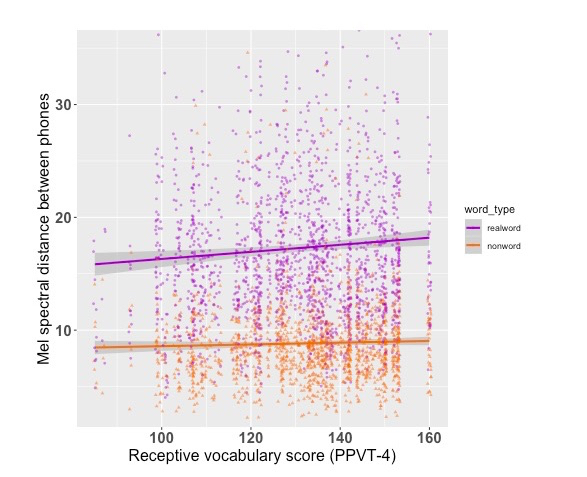
\includegraphics[scale=.7]{figures/figure_1.jpeg}
\caption{\label{fig:figure-1}CV coarticulation by receptive vocabulary score (PPVT-4)}
\end{figure}




\begin{table}[!htbp] \centering 
  \caption{The effects of vocabulary and word duration upon coarticulation} 
  \label{tab:model-1} 
\begin{tabular}{@{\extracolsep{5pt}}lc} 
\\[-1.8ex]\hline 
\hline \\[-1.8ex] 
 Intercept & 6.67$^{***}$ \\ 
  & (5.06, 8.28) \\ 
  & t = 8.13 \\ 
  & p = 0.00 \\ 
  Receptive vocabulary score (PPVT-4) & 0.02$^{**}$ \\ 
  & (0.004, 0.03) \\ 
  & t = 2.65 \\ 
  & p = 0.01 \\ 
  Word duration (ms) & 0.001$^{*}$ \\ 
  & (0.0000, 0.001) \\ 
  & t = 2.02 \\ 
  & p = 0.05 \\ 
 \hline \\[-1.8ex] 
Log Likelihood & $-$9,163.64 \\ 
Akaike Inf. Crit. & 18,339.27 \\ 
Bayesian Inf. Crit. & 18,376.15 \\ 
\hline 
\hline \\[-1.8ex] 
\textit{Note:}  & \multicolumn{1}{r}{$^{*}$p$<$0.05; $^{**}$p$<$0.01; $^{***}$p$<$0.001} \\ 
\end{tabular} 
\end{table}


\subsection{Spoken language experience and coarticulation}

After evaluating the roles of speech planning and vocabulary size for coarticulation, we turned to how speech practice may predict the children’s speech patterns and, more specifically, how speech practice could interact with speech planning and vocabulary. We predicted that the frequency of children’s vocalizations, quantified in daylong audio recordings, would mediate their coarticulation patterns: children who vocalize more often in daylong recordings will coarticulate less within CV sequences. To evaluate this hypothesis, an additional mixed effects linear regression model was fit to predict the Mel spectral distance between phones in each CV sequence. As before, a larger spectral distance indicates less gestural overlap---less coarticulation---between the segments.

To address the role of speech practice on coarticulation, we included measures of the children’s daily language experiences from the 80 of the 103 children (77.7\%) who completed a daylong audio recording that was at least 9 hours long. The baseline model included the random effects of Word and Participant. We then repeated the forward model fitting procedure as before with the following parameters added: Word Duration, Phonotactic Transitional Probability, Second Syllable Frequency, Word Type, Late Talker, Maternal Education Level, Gender, Receptive Vocabulary Size (PPVT-4 growth scale value), Expressive Vocabulary Size (EVT-2 growth scale value), and Child Vocalization Count (the average number of hourly child vocalizations from the daylong recording). Predictors that did not improve model fit were removed from the analysis. 

As in the model fit to the full dataset, Phonotactic Transitional Probability, Second Syllable Frequency, and Word Type did not improve upon a baseline model fit with just the random effects and Word Duration. We likewise did not find significant model improvements after adding Maternal Education Level, Gender, or Late Talker so we removed those factors from the model. 

Table \ref{tab:model-2} shows the final model fit with significant main effects of Word Duration and Expressive Vocabulary Size (β=.02, t=2.57, p=0.01).\footnote{In the dataset containing children who completed a daylong recording, Expressive Vocabulary Size proved a marginally better fit than Receptive Vocabulary Size. This fact further underscores the lack of distinction between Expressive and Receptive Vocabulary Sizes for coarticulation: we do not find strong evidence for one vocabulary measure over the other.} Child Vocalization Count was also significant, indicating that children who tended to vocalize more throughout the daylong recording coarticulated less within CV sequences (β=.003, t=2.74, p=0.01), whether the sequences were embedded in nonwords or real words (Figure \ref{fig:figure-2}). This result provides some support for a ``practice effect'' for children’s coarticulation patterns.

Child Vocalization Count and Receptive Vocabulary Size were not significantly correlated (Pearson r=.02, t=.16, p=.88). Nor were Child Vocalization Count and Expressive Vocabulary Size (r=-0.05, t=-0.47, p=.64). This lack of correlation between these variables indicates that children’s language skills and vocabulary sizes do not simply increase as they talk/vocalize more frequently, a point which is further addressed in the Discussion.

To further explore the patterns between vocabulary, child vocalizations, and coarticulation, we performed a median split on the 80 children who had completed a daylong recording, dividing them into smaller (n=52 children) and larger expressive vocabulary groups (n=28 children). Dividing the children into these groups allowed us to see that the effect of Child Vocalization Count appears to be especially prominent for the children in the smaller vocabulary group (left panel of Figure \ref{fig:figure-2}). For the children with larger vocabularies, Child Vocalization Count does not appear to be strongly correlated with coarticulation. Despite these differences by vocabulary size, the interaction of Child Vocalization Count and Expressive Vocabulary was not significant.  Finally, while the relationship between Child Vocalization Count and coarticulation may have been weaker in the larger vocabulary group the effect of word type---though not significant in the modeling---appears to be stronger in the larger vocabulary group. Children with larger vocabularies tend to coarticulate just slightly more in nonwords than real words. This is, however, just a trend in the data as the interaction of Word Type and Expressive/Receptive Vocabulary Sizes was not significant. 


\begin{figure}[H]
\centering
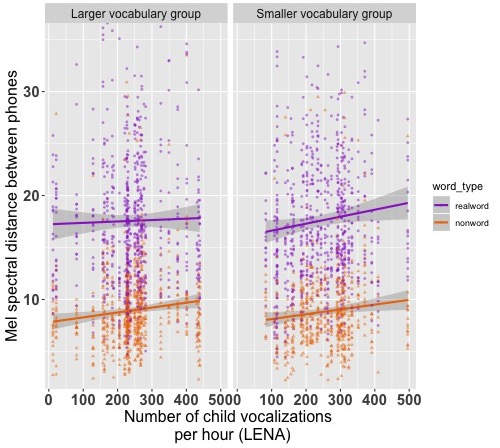
\includegraphics[scale=.7]{figures/figure_2.jpeg}
\caption{\label{fig:figure-2}Child vocalization count by Mel spectral distance between CV phones with a median split by expressive vocabulary size (EVT-2).}
\end{figure}



\begin{table}[!htbp] \centering 
  \caption{The effects of speech practice and vocabulary upon coarticulation} 
  \label{tab:model-2} 
\begin{tabular}{@{\extracolsep{5pt}}lc} 
\\[-1.8ex]\hline 
\hline \\[-1.8ex] 
 Intercept & 7.99$^{***}$ \\ 
  & (7.20, 8.79) \\ 
  & t = 19.71 \\ 
  & p = 0.00 \\ 
  Hourly child vocalization count & 0.003$^{**}$ \\ 
  & (0.001, 0.01) \\ 
  & t = 2.74 \\ 
  & p = 0.01 \\ 
  Word duration (ms) & 0.001$^{*}$ \\ 
  & (0.0001, 0.001) \\ 
  & t = 2.43 \\ 
  & p = 0.02 \\ 
  Expressive vocabulary score (EVT-2) & 0.02$^{*}$ \\ 
  & (0.005, 0.04) \\ 
  & t = 2.57 \\ 
  & p = 0.02 \\ 
 \hline \\[-1.8ex] 
Log Likelihood & $-$7,454.78 \\ 
Akaike Inf. Crit. & 14,923.57 \\ 
Bayesian Inf. Crit. & 14,965.08 \\ 
\hline 
\hline \\[-1.8ex] 
\textit{Note:}  & \multicolumn{1}{r}{$^{*}$p$<$0.05; $^{**}$p$<$0.01; $^{***}$p$<$0.001} \\ 
\end{tabular} 
\end{table} 


\subsection{Language input and coarticulation}

Although we found that children who vocalized more in the daylong recordings coarticulated less within the CV sequences, these results could also be explained by parent-child engagement. Specifically, children who hear more input from caregivers may, in turn, speak more so there could be an indirect role of input upon children's coarticulation. In our sample, we did find that the average number of hourly child vocalizations was positively correlated with the average number of hourly adult words (r=.44, t=4.35, p<.001; Figure \ref{fig:figure-3}). This positive correlation between the two measures led us to hypothesize that the quantity of adult speech in the child’s environment could predict the child’s coarticulation patterns, potentially having a stronger role than the child’s own productions. 


\begin{figure}[H]
\centering
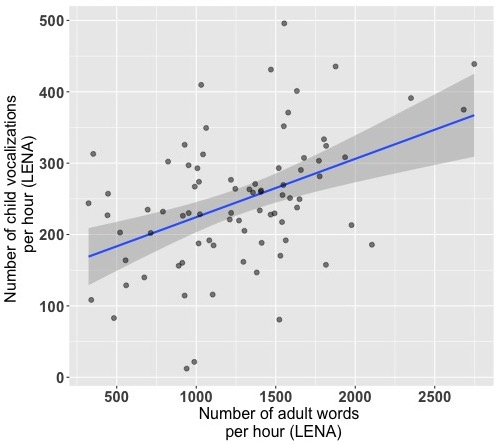
\includegraphics[scale=.8]{figures/figure_3.jpeg}
\caption{\label{fig:figure-3}Relationship between adult word count and child vocalization count}
\end{figure}

We tested this exploratory hypothesis in the same model of the 80 children who completed a daylong recording. Now instead of adding Child Vocalization Count, we instead added Adult Word Count, or the average number of words spoken by adults per hour in the daylong recording. Adult Word Count did not improve model fit, either with a model that included Child Vocalization Count ($\chi$\textsuperscript{2}=1.99, df=1, p=.16) or one that did not ($\chi$\textsuperscript{2}=.01, df=1, p=.92). Therefore, we can confidently conclude that Adult Word Count does not directly predict children’s coarticulation within the CV sequences.

While we did not find a direct effect of Adult Word Count, the relationship between Adult Word Count and Child Vocalization Count, and in turn the relationship between Child Vocalization Count and degree of coarticulation, suggests an indirect role of Adult Word Count on children’s coarticulation: more adult words spoken in the environment leads to a greater number of child vocalizations, which, in turn, predicts the degree of children’s coarticulation. This relationship between the quantity of ambient adult language and coarticulation is indirect: Adult Word Count is not related to the children’s coarticulatory outcomes without factoring in Child Vocalization Count.  

\subsection{Coarticulation by consonant manner}

The acoustic measure employed here is validated for all consonant manners. However, we additionally analyzed the potential effect of consonant manner on the relationship between coarticulation, vocabulary size, and child vocalizations. In all cases, analysis was limited to glides, fricatives, and stops because there was only 1 stimulus pair with an affricate-vowel sequence. Broadly, the results by consonant manner replicated those conducted over all segments together: there was little to no effect of word type (Figure \ref{fig:figure-4} in Appendix A) and children with larger vocabularies tended to coarticulate less. The vocabulary effect was most pronounced in fricative-vowel and glide-vowel sequences. Children who vocalized more also tended to coarticulate less between CV sequences, independent of consonant manner (Figure \ref{fig:figure-5} in Appendix A). 

\section{Discussion}

\subsection{Coarticulation in real words and nonwords}

Previous work has primarily attributed young children’s propensity to coarticulate to two factors: children’s immature, developing speech motor control \cite{barbierWhatAnticipatoryCoarticulation2020,rubertusDevelopmentGesturalOrganization2018,zharkovaDynamicsVoicelessSibilant2018} and the size of their representational units \cite{nittrouerEmergencePhoneticSegments1989,nittrouerHowChildrenLearn1996,noiraySpokenLanguageDevelopment2019,zharkovaCoarticulationIndicatorSpeech2011}. Past work has used cross-sectional experimental designs to distinguish between motoric and representational explanations for coarticulation. But children's motor skills are tightly tied to their chronological age. This study instead evaluated how several factors---speech planning, vocabulary size, and speech practice---could predict coarticulation in a large cohort of four-year-old children.  Crucially, each of these factors develops more independently of speech motor control than children's age. Thus, evaluating the relationships between these factors and the degree of children’s coarticulation allows us to determine some additional, underlying causes of coarticulation, beyond children’s developing motor control abilities. In the following sections, we discuss our findings concerning each of the three factors and their relationship with four-year-old children’s coarticulation patterns. 

To evaluate the role of speech planning, the degree of the children’s coarticulation was measured in two environments: real words and corresponding nonwords (e.g. [su] in \textit{suitcase} and \textit{sudras}). We hypothesized that children would coarticulate less between CV sequences embedded in real words than nonwords because children have more experience accessing and articulating the real words making nonword repetition a more demanding task. For example, while the CV sequence was matched across each real word and nonword pair, nonword production requires repetition without any phonetic, lexical, or semantic support. Speakers must encode and produce a novel combination of syllables without reinforcement. In real word repetition, on the other hand, speakers encode a semantic and phono-lexical representation and then execute the associated articulatory schema. Nonword repetition is also often considered a proxy for phonological representations in working memory (e.g. \citeNP{edwardsNonwordRepetitionsChildren1998,gathercoleNonwordRepetitionWord2006}): children with larger vocabularies perform better on the task \cite{edwardsInteractionVocabularySize2004,munsonRelationshipsNonwordRepetition2005} and speakers of all ages perform worse on longer, multisyllabic words \cite{byrdNonwordRepetitionPhoneme2012}.\footnote{Nonword repetition is a proxy for phonological working memory, but there are myriad factors, including those pertaining to the stimuli like phoneme frequency and sub-syllabic frequency, that predict task performance (see \citeauthor{szewczykNonwordRepetitionDepends2018} (2018) for comprehensive overview).} The task demands of nonword repetition, in addition to the fact that children cannot rely upon established motor schemata to articulate the nonwords, could then affect the children’s coarticulation by not permitting the same degree of planning permitted for real word repetition. 

Our analyses did not support the prediction that children would coarticulate more in nonwords: there was no effect of word type on coarticulation after controlling for word duration. Children with larger expressive vocabularies did tend to coarticulate less between CV sequences in real words than nonwords, but this did not approach significance in the modeling. There are several ways to interpret this result. First, there could simply be no effect of speech planning on children's coarticulation. Second, there could be an effect of speech planning but it is only apparent under certain experimental manipulations and lexical status is not one of them. Finally, there could be an effect of speech planning on coarticulation as implemented in this experimental design, but the much stronger effect of speaking rate on coarticulation may have masked the weaker, correlated effect of word type. We address this possibility in the remainder of this section.

Word duration was controlled for in the modeling both because the nonwords tended to be longer in duration than the real words and also because, more generally, coarticulation and speaking rate are tightly linked. Adult speakers coarticulate more in faster speech \cite{gayMechanismsControlSpeech1981,matthiesVariationAnticipatoryCoarticulation2001}. The relationship between coarticulation and speaking rate may be reversed in children whose coarticulation reflects different pressures.   In adults, coarticulation is usually planned \cite{whalenCoarticulationLargelyPlanned1990} and reflects an equilibrium between speaker efficiency and listener comprehension \cite{bradlowConfluentTalkerListeneroriented2002}. But, as stated throughout this work, child coarticulation is instead generally attributed to a lack of fine motor control and entrenched articulatory schema that may be required to differentiate between adjacent phones during speech \cite{goffmanRelationsSegmentalMotor2007,greenPhysiologicDevelopmentSpeech2000,mcallisterbyunMotorInfluencesGrammar2016} or phonological reorganization \cite{nittrouerEmergencePhoneticSegments1989,nittrouerHowChildrenLearn1996,noiraySpokenLanguageDevelopment2019,redfordGrammaticalWordProduction2018,zharkovaCoarticulationIndicatorSpeech2011}. The result is that children might coarticulate more in \textit{slower} speech; but their coarticulation and speaking rate are, nevertheless, intertwined. 

Because of this relationship between speaking rate and coarticulation, it was essential to include a proxy for speaking rate (word duration) in the modeling. However, word duration, which covaries tightly with word type,  might have masked any effect of word type. There are two reasons why word duration would have this effect. First, the effect of speaking rate on coarticulation is quite robust \cite{gayMechanismsControlSpeech1981,matthiesVariationAnticipatoryCoarticulation2001}, regardless of the direction of the effect by age. Second, any effect of word type on degree of coarticulation is likely to be quite small. Even employing a fine-grained measure of coarticulation such as that used here might not be capable of capturing differences due to word type that are independent of the strong link between word duration and coarticulation. 

We summarize the results of speech planning on coarticulation by saying that there is no reliable effect of word type upon coarticulation that is independent of speaking rate. An effect of word type would have provided evidence of extra-motoric influences on coarticulation, such as those stemming from phonological reorganization. In the following sections we interpret the findings from the other two variables studied, vocabulary size and speech practice, which do suggest an effect of phonological reorganization upon children's coarticulation. 

\subsection{Language experience and coarticulation}

\subsubsection{The role of vocabulary size on coarticulation}

Our second hypothesis concerned the role of vocabulary size on child coarticulation patterns in the real words and nonwords. Using our full sample size of 103 children, we found that children with larger receptive vocabularies coarticulated less between the segments in CV sequences. Receptive vocabulary size was only marginally more predictive of coarticulation degree than expressive vocabulary size for the full dataset. The difference between the models with the different vocabulary measures was marginal. Furthermore, expressive and receptive vocabulary scores are correlated, and in the sub-analysis of the 80 children who completed a daylong recording, we instead found that expressive vocabulary better predicted coarticulation outcomes. As a result, we do not make strong claims concerning the role of receptive versus expressive vocabulary for coarticulation: both estimates predict coarticulation to a relatively similar degree.

Given the results of \citeauthor{noiraySpokenLanguageDevelopment2019} (2019), the finding in this paper that children with larger vocabularies coarticulate less is unsurprising. \citeauthor{noiraySpokenLanguageDevelopment2019} (2019) evaluated a relationship between vocabulary size and degree of coarticulation in children aged 4;0-7;0 and found that children with larger expressive vocabularies showed less anticipatory coarticulation in [stop]-V sequences. The results from the current paper replicate this finding. \citeauthor{noiraySpokenLanguageDevelopment2019} (2019) attributed the relationship between vocabulary size and coarticulation to the primacy of the lexicon for phonetic and phonological development as phonological representations emerge from generalizations that children make over their vocabularies.  This theoretical approach argues that as the lexicon grows, phonological representations reorganize from larger sub-lexical units like syllables and feet into smaller, phoneme-sized ones \cite{beckmanGeneralizingLexiconsPredict2010,edwardsInteractionVocabularySize2004,metsalaYoungChildrenPhonological1999,metsalaSpokenVocabularyGrowth1998,storkelInfluencePartwordPhonotactic2011,storkelLexiconPhonologyInteractions2002}. Children with larger vocabularies are then expected to have more abstract speech segments. Phonological reorganization manifests in production accuracy when children with larger vocabularies perform better on nonword repetition (3;2-8;10: \citeNP{edwardsInteractionVocabularySize2004}; 3;0-6;0: \citeNP{munsonRelationshipsNonwordRepetition2005}) and novel word learning tasks (2;11-6;0: \citeNP{storkelInfluencePartwordPhonotactic2011}). The phonological abstraction stemming from the growth of the lexicon could also play out in children’s phonetic development as children with larger vocabularies coarticulate less. Still, the relationship between receptive vocabulary size and coarticulation observed here is not as robust as the relationship between vocabulary size and those other outcome measures (repetition accuracy, novel word learning) \cite{edwardsInteractionVocabularySize2004,metsalaYoungChildrenPhonological1999,storkelInfluencePartwordPhonotactic2011}. The different result found here could be because there are myriad other factors, beyond vocabulary size, that predict children’s spoken phonetic outcomes, and coarticulation in particular. 

Throughout this work, we have entertained two primary explanations for children’s coarticulation patterns: speech motor control and phonological reorganization. The finding that children with larger vocabularies coarticulate less supports the idea that coarticulation reflects phonological reorganization from larger sub-lexical units into phonemes because previous work has concluded that children with larger vocabularies have more segmental phonological representations (e.g. \citeNP{metsalaSpokenVocabularyGrowth1998}). However, the weaker relationship between coarticulation and vocabulary size, compared to previous work evaluating the relationship between word learning or repetition accuracy and vocabulary size, suggests that there is also a strong role of another factor for children’s coarticulation---fine motor control---that may not explain as much variability in novel word learning or nonword repetition accuracy. Vocabulary size may predict coarticulation, but the effect is weaker because fine motor control exerts a strong influence on phonetic outcomes \cite{barbierWhatAnticipatoryCoarticulation2020} in a way that it does not for word learning and other lexical tasks.

\subsubsection{The role of production practice on coarticulation}

The final potential predictor of children’s coarticulation that we evaluated in this study was the frequency of children’s vocalizations. The role of children's vocalization frequency was examined in the subset of children who completed a daylong audio recording (80/103 or 77.7\%) and we found that children who vocalized more during the daylong recording coarticulated less, both in real words and nonwords. This study was the first to examine this ``practice effect'' in older children, aged 4;0, using naturalistic recordings of the children’s everyday environments. Our results corroborate previous evidence in support of a practice effect for speech development (\citeNP{depaolisProductionPatternsInfluence2011,depaolisInfluenceBabblingPatterns2013,ichtProductionEffectMemory2015,keren-portnoyRoleVocalPractice2010,majoranoRelationshipInfantsProduction2014,redford2014} cf. \citeNP{zamunerReverseProductionEffect2018}) whereby children who practice more spoken language, or articulate words during word learning, could learn to encode articulatory movements with their acoustic representations. This articulatory practice, in turn, may further entrench phonological representations and may make the task of accessing a given word or phone easier, and smoother, for future productions. The results found here also support previous findings on a different measure of children's speech practice---articulation rate. That work has demonstrated how adults perceive children who speak faster to have clearer speech, again suggesting that children who talk more have more mature speech production outcomes \cite{redford2014}.\footnote{Given the results of \citeauthor{redford2014} (2014), a supplementary analysis was performed to evaluate the relationship between articulation rate (duration of repeated words) and Child Vocalization Count for the children in the current study who completed a daylong recording. Results showed a significant, but weak correlation between the duration of the repeated real words and Child Vocalization Count (r= -.07, t= -2.72, p=0.007) suggesting that children who speak more throughout the day also speak faster, at least in a lab-based word repetition task (there was no relationship between the duration of nonwords and Child Vocalization Count).} 

The practice effect found here is potentially even more interesting since it works independently from vocabulary size: we did not find a positive relationship between children's vocalization frequency and their vocabulary size. The lack of a relationship between vocalization frequency and vocabulary size suggests  that speech practice predicts speech development without the mediating factor of vocabulary size. 

It should be noted that our estimate of hourly child vocalizations was relatively coarse. While the child vocalization count estimator of the LENA speech parsing algorithm performs reliably well \cite{cristiaThoroughEvaluationLanguage2020} (better than other more language- and context-specific estimations from LENA), the algorithm does not distinguish between speech-like vocalizations and crying or laughing. Consequently, this study is an important first step in establishing the role of self-practice for children’s coarticulation and speech development. Future work now needs to evaluate children’s naturalistic speech productions in this age range in a more fine-grained manner to better understand what characteristics of children’s vocalizations predict their speech outcomes. For example, while we did not find that an estimate of receptive language experience, adult word count, directly predicted the degree of coarticulation, adult word count and child vocalization count were positively correlated. Thus, it could be that interactions with adult interlocutors in particular indirectly predict coarticulatory development. Delving deeper into the role of self-practice and the language learning environment is thus an important area for future research on phonetic development. 

This study only measured coarticulation between CV sequences in words that the children repeated correctly. Words in which the children made phonological substitutions or deleted syllables were removed from analysis. The decision to remove incorrect words was made for practical reasons: there was no way to control the errors that children made as they repeated the words, which made it difficult to perform an individual differences analysis. However, children probably do coarticulate differently in words that they repeat incorrectly. For example, deletion of a syllable during word repetition could indicate that greater planning demands were placed on the child, meaning they might have been more likely to coarticulate. For substitution errors, children who regularly substitute [w] for /r/ might coarticulate more in [we] sequences in words like ``raisin'' than they do in phonemically /we/ sequences in words like ``wait'' or ``waste.'' Consequently, measuring coarticulation in correctly- and incorrectly-repeated words seems to be a potentially informative line of future research on speech development which we encourage on the basis of the results from correctly-repeated words in the current study. 

\subsection{On data exclusion and daylong recordings}

As daylong recording methodologies increase in popularity in developmental language research, ethical issues surrounding participant exclusion will become more apparent \cite{casillasStepbystepGuideCollecting2019}. In this study, 22 families opted not to participate in the daylong recording portion of the study. We still included the word repetition and vocabulary data for these children rather than excluding them completely from the study. 

Daylong recordings require that children wear recorders over extended periods. Sound within an approximately five foot radius of the child is captured in the recording. Some families may, understandably, not be comfortable with this methodology. One solution for studies like ours that incorporate covariates derived from daylong recordings could be to exclude all children whose families opt out of the daylong recording. However, we do not encourage this option. The decision to contribute a daylong audio recording to a research study may depend on several external factors like socioeconomic status, race, and familial structure (i.e. single-parent households). For example, in a hypothetical example that relates to the current study, some caregivers may have unpredictable work schedules making it difficult to complete a 12 hour recording. Given these challenges, it would hardly be surprising if some individuals from under-served communities were more likely to opt out of daylong recording methodologies. In fact, in our sample, we found a different SES distribution in families who completed the daylong recording (92.59\% of mothers had more than a high school diploma) versus those who did not (86.36\% of mothers had more than a high school diploma).\footnote{ The SES breakdown of the two groups was as follows: for families who did complete a daylong recording n=1 did not have a high school diploma, n=1 had the equivalent of a high school diploma (e.g. GED), n=4 had a high school diploma, n=0 had <2 years of college, n=15 had 2+ years of college, n=27 had completed college, and n=33 had graduate degrees . For families who did not complete a daylong recording, n=1 did not have a high diploma, n=0 had the equivalent of a high school diploma, n=2 had a high school diploma, n=1 had <2 years of college, n=6 had 2+ years of college, n=6 had completed college, and n=6 had graduate degrees.} Thus, excluding all families who could not complete a daylong recording could inadvertently exclude some groups from representation in social science research. The exclusion of these families would not be random and could, inadvertently, serve to further bias language development findings for upper middle class North American children. 

\subsection{The status of children’s phonological representations}

An overarching goal of this study was to contribute to our understanding of children’s phonological representations. By showing novel evidence for the roles of vocabulary size and speech practice---but not speech planning---on coarticulation, this study corroborates \citeauthor{noiraySpokenLanguageDevelopment2019} (2019) in suggesting that coarticulation is dually explained by speech motor control maturation and phonological reorganization. In particular, the predictive relationship of vocabulary size for coarticulation found in this study suggests that children with larger lexicons have more segmental phonological units. This finding supports phonological reorganization. 

The ramifications for the role of child vocalization frequency may be less straightforward because algorithmically-derived speech measures, such as LENA’s child vocalization count or adult word count, do not necessarily map onto linguistically-coded categories. Children who vocalized more often during the daylong recording may exhibit motor practice effects, resulting in more entrenched or even abstracted phonological categories. Of course children who vocalize more could also have greater motor control because they speak more frequently. The hourly child vocalization count derived from the LENA recordings was more predictive than vocabulary size (receptive or expressive) for coarticulation in the participants where we could test both vocabulary size and child vocalization count. On the basis of the comparison of these two factors, it appears that the frequency of speech practice is the strongest predictor of children’s coarticulation patterns. 

\section{Conclusion}

This study measured four-year-old children’s coarticulation between phones in CV sequences. Previous work on this topic has struggled to disentangle the roles of fine motor control and the potential role of children’s larger representational units for children’s coarticulation patterns. Three factors that develop more independently of fine motor control than children's age---speech planning, vocabulary size, and speech practice---were evaluated for their role on coarticulation. We did not find an effect of speech planning on coarticulation: children coarticulated similarly in real words and matched nonwords after controlling for speaking rate. We did, however, find effects of vocabulary size and speech practice. Children with larger vocabularies coarticulated less, as did those who vocalized more during a daylong audio recording. This daily practice effect was more predictive of coarticulatory outcomes than the quantity of adult language in the ambient environment and the child's vocabulary size, suggesting the strong role of self-practice for speech development. Overall, the observed effects of vocabulary size and speech practice suggest that both fine motor control and children's representational units independently explain the development of coarticulation. (Word count: 11955)

\section{Acknowledgements}

The authors wish to acknowledge the families who participated in this research. We also thank many members of the Learning to Talk Labs at the University of Wisconsin, Madison and the University of Minnesota, Twin Cities for assistance with data collection. Additional thanks to Rebecca Higgins at the University of Maryland, College Park for her assistance in data processing. This research was supported by the Raymond H. Stetson Scholarship in Phonetics and Speech Science (M.C.) and National Institute on Deafness and Other Communication Disorders Grant T32DC000046 (M.C.) and R0102932 (J.R.E., B.M., and Mary E. Beckman).   

\section{Declaration of interest}

The authors have no conflicts of interest to report. 



\bibliography{zotero_library}

\begin{figure}[H]
\centering
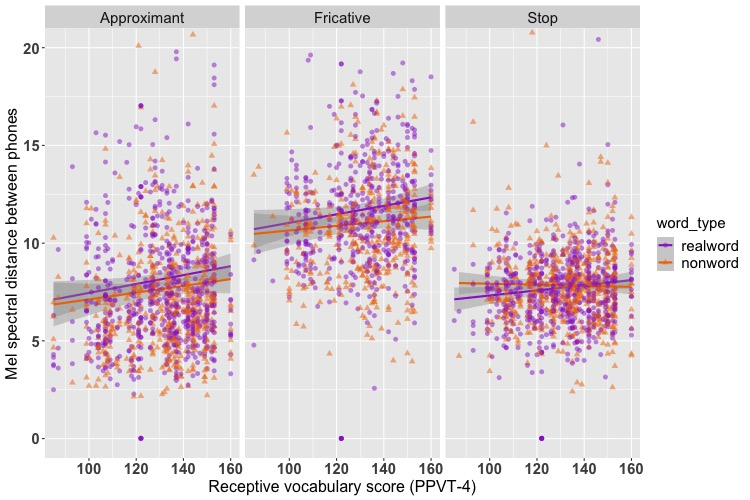
\includegraphics[scale=.7]{figures/figure_4.jpeg}
\caption{\label{fig:figure-4}CV coarticulation by receptive vocabulary size and consonant manner}
\end{figure}

\begin{figure}[H]
\centering
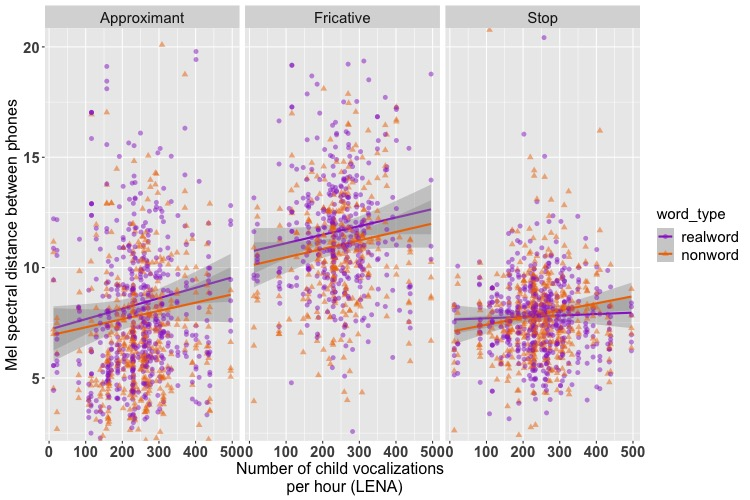
\includegraphics[scale=.7]{figures/figure_5.jpeg}
\caption{\label{fig:figure-5}CV coarticulation by number of child vocalizations and consonant manner}
\end{figure}

\end{document}